En el campo de la robótica móvil, la navegación autónoma desempeña una tarea fundamental para que los sistemas robóticos se desplacen de manera segura y eficiente en entornos dinámicos y desconocidos. Este proceso implica la percepción del entorno mediante sensores, la planificación y ejecución de trayectorias y la toma de decisiones en tiempo real, sin la necesidad de intervención humana directa. Por lo tanto, la exitosa integración de este proceso resulta en una mayor capacidad de adaptación y desempeño de los robots móviles con su entorno, promoviendo la autonomía e independencia de estos sistemas.

\section{Generación de trayectorias y mapeo de entornos}
En \cite{li_map_2023} se describió un método de construcción para mapeo de entornos basado en un mapa de cuadrícula de probabilidad de colisión y la mejora de un algoritmo A*. Se utilizaron técnicas de probabilidad de colisión que consideraron tanto el tamaño del robot como la posición relativa de este y los obstáculos presentes en la cuadrícula para construir un mapa del entorno. El método permitió encontrar rutas seguras y eficientes al integrar información de probabilidad de colisión en el proceso de construcción de mapas y planificación de rutas desde el nodo de inicio hasta el nodo objetivo. El mapa generado ofrece una cuadrícula en escala de grises indicando la probabilidad de colisión según la cercanía de los obstáculos; cuanto más oscuro el color, más peligroso y cercano se encuentra el obstáculo. En cambio, la cuadrícula blanca representa la zona libre y menos propensa a la colisión.

\begin{figure}[H]
	\centering
	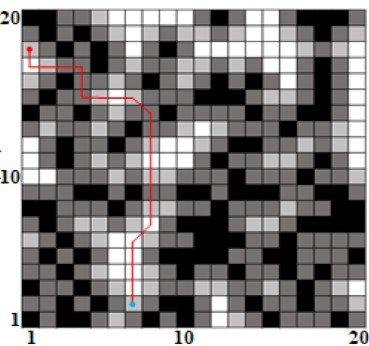
\includegraphics[width=0.45\textwidth]{mapa_colisiones.jpg}
	\caption{Mapa generado a partir de cuadrícula de probabilidad de colisión con ruta óptima \cite{li_map_2023}.}
	\label{fig2_1}
\end{figure}

Además, considera la función de costo del algoritmo A*, minimizando el tiempo de búsqueda de nodos peligrosos en entornos complejos, generando un mapa más completo y reduciendo el tiempo de búsqueda y número de giros en las rutas propuestas. Los resultados de las simulaciones realizadas en Matlab demuestran mejoras en la seguridad ante colisiones y eficiencia de localización de objetos en entornos complejos sobre algoritmos tradicionales. Sin embargo, los autores identifican ciertas limitaciones ante obstáculos dinámicos al momento de mapear el entorno.\\

En \cite{li_quadruped_2022} se desarrolló e implementó un algoritmo para el mapeo bidimensional en robots cuadrúpedos utilizando estimaciones de mínimos cuadrados. El algoritmo generado tuvo como finalidad planificar y producir trayectorias de seguimiento que permitieron la evasión de obstáculos en entornos cambiantes. Esto se logró por medio de un radar láser 3D y un sistema de posicionamiento de banda ultraancha (UWB) los cuales proporcionaban datos espaciales y direccionales del entorno en tiempo real. Dicha información fue transformada en un mapa de rejilla 2D donde se estableció la ubicación actual del cuadrúpedo, la presencia de obstáculos y los espacios libres de movimiento. El artículo presentó resultados experimentales que demostraron la precisión del algoritmo en la construcción del entorno y la autonomía del cuadrúpedo al ajustar sus movimientos y trayectorias en tiempo real según diferentes situaciones. Además, se destacó la futura implementación de algoritmos de trayectorias globales y locales para mejorar la reconstrucción del entorno y la estabilidad del sistema de planificación de rutas y navegación espacial.

\section{\textit{Ant Colony Optimization} (ACO)}

En \cite{dai_mobile_2019} se compararon algoritmos basados en ACO para abordar la problemática de planificación de rutas para robots móviles en entornos complejos. En el artículo se analizaron diferentes parámetros para determinar tanto la convergencia de las trayectorias como la optimización y suavidad de las rutas en diferentes entornos de simulación para cada uno de los algoritmos propuestos. Además, se destacó la implementación de mecanismos de reacción y supresión de curvas para mejorar el rendimiento y adaptabilidad de estos, resultando en un algoritmo que superó en eficiencia y convergencia las versiones tradicionales de ACO. Los resultados de simulación en MATLAB demostraron que el algoritmo mejorado garantiza que los robots puedan encontrar una trayectoria satisfactoria incluso en situaciones desafiantes.


\begin{figure}[H]
	\centering
	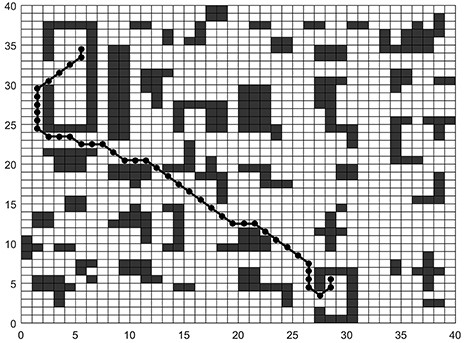
\includegraphics[width=0.6\textwidth]{ruta_algoritmo_mod.jpg}
	\caption{Ruta generada a partir del algoritmo ACO mejorado \cite{dai_mobile_2019}.}
	\label{fig2_2}
\end{figure}

\section{\textit{Particle Swarm Optimization} (PSO)}
En \cite{han_mobile_2019} se presentó la implementación de PSO para la planificación de rutas de robots móviles en coordenadas polares. Se empleó el algoritmo de optimización por enjambre de partículas como un proceso de búsqueda donde cada agente se movió a través de un espacio bidimensional buscando la mejor ruta desde el punto de inicio hasta el punto objetivo. Durante la ejecución del algoritmo, los agentes se movieron a través del espacio de búsqueda, ajustando su posición y velocidad en función de la información obtenida de su propio desempeño pasado y de la mejor solución global encontrada por otros agentes en el enjambre. Este proceso de búsqueda colectiva permitió que los agentes exploraran el espacio y convergieran hacia soluciones óptimas. Los resultados de simulación demostraron que el algoritmo PSO eliminó puntos de ruta redundantes, optimizando la eficiencia de trayectorias planificadas. Sin embargo, los autores identificaron ciertas limitaciones de escalabilidad en entornos con obstáculos dinámicos. 

\section{Implementación de algoritmos de inteligencia de enjambre en UVG}
En el trabajo de investigación \cite{pena_echeverria_algoritmo_2019} se desarrolló e implementó un algoritmo de control para sistemas de robots multi-agente orientado a misiones de búsqueda, basado en métodos teóricos de grafos y control moderno. Se destacó que la integración de una sola función racional que combina el control de formación y colisiones permitía que los agentes alcanzaran formaciones con un mínimo error cuadrático medio al utilizar grafos totalmente rígidos. Además, los resultados de la simulación en el entorno de Webots demostraron que los agentes lograron alcanzar la meta en el 80\% de los escenarios considerados, con un 11\% de éxito en control de formación. Esto indicó que el algoritmo propuesto fue efectivo en la coordinación de los agentes, más no fue eficiente en la cantidad de formaciones finales exitosas.

\begin{figure}[H]
	\centering
	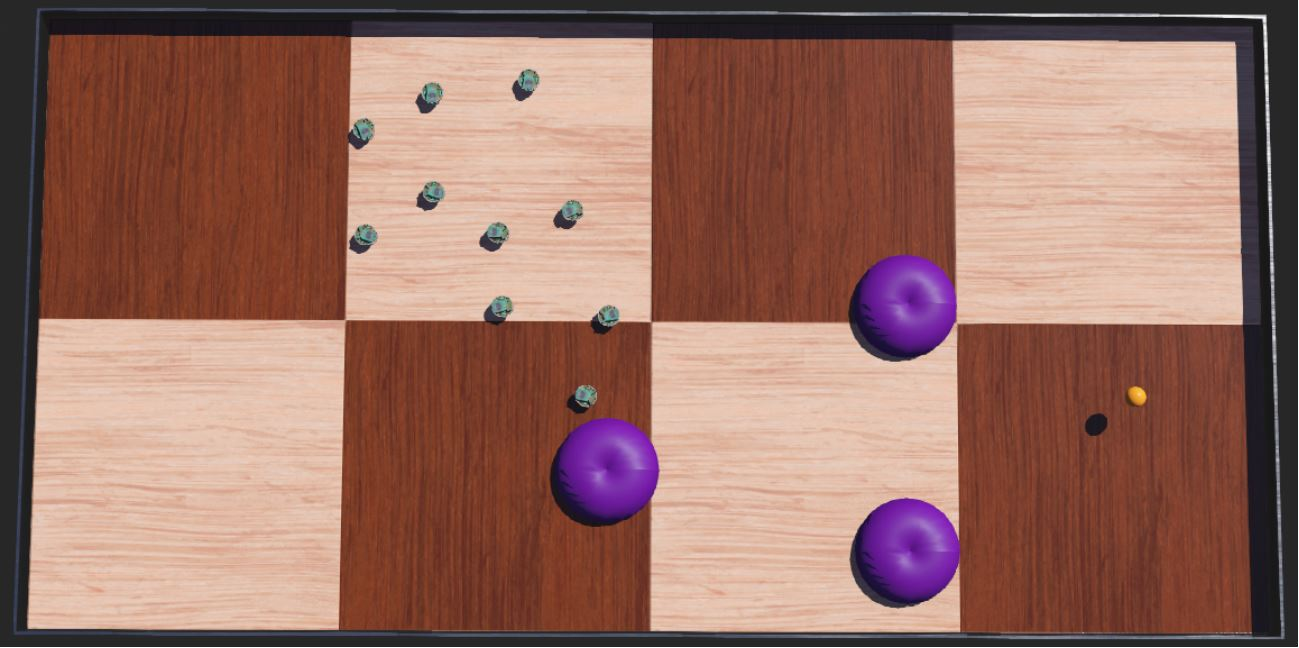
\includegraphics[width=0.75\textwidth]{desplazamiento.jpg}
	\caption{Desplazamiento del grupo de robots hacia la meta  \cite{pena_echeverria_algoritmo_2019}.}
	\label{fig2_3}
\end{figure}

\begin{figure}[H]
	\centering
	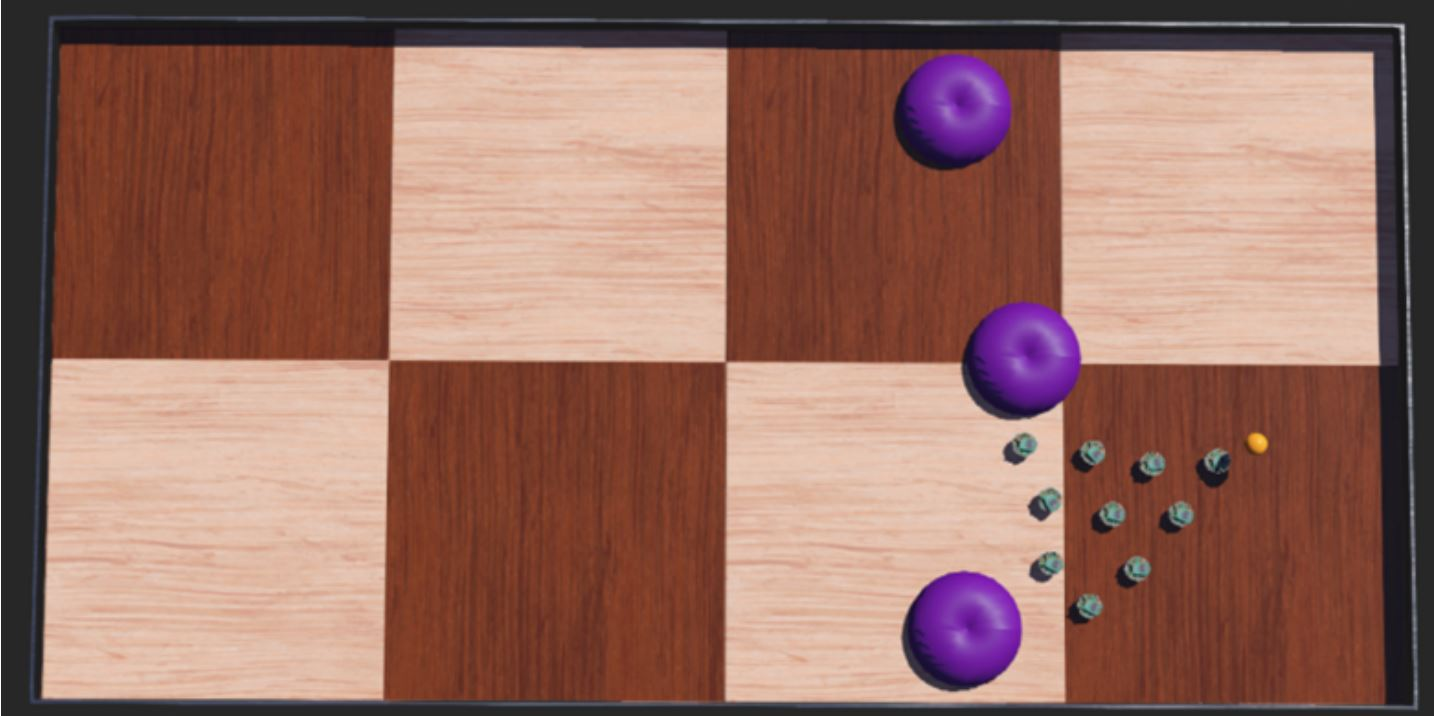
\includegraphics[width=0.75\textwidth]{formacion.jpg}
	\caption{Formación triangular del grupo de robots en la meta \cite{pena_echeverria_algoritmo_2019}.}
	\label{fig2_4}
\end{figure}

En \cite{santizo_olivet_aprendizaje_2021} se desarrolló un algoritmo que determinaba los parámetros más adecuados para mejorar y potenciar el desempeño del algoritmo PSO estándar. Mediante el uso de redes neuronales recurrentes, la herramienta nombrada Deep PSO Tuner, permitió la selección dinámica y automática de los hiper-parámetros que debería de emplear el algoritmo, mejorando la precisión y tiempo de convergencia del mismo. Los resultados de las simulaciones realizadas demostraron que la red nueronal BiLSTM fue la más efectiva, logrando superar obstáculos locales y permitiendo una mayor precisión y rendimiento del algoritmo en diferente situaciones. No obstante, se mencionaron ciertas limitaciones respecto a la escalabilidad del método y la baja reacción del algoritmo en situaciones con obstáculos dinámicos.

En el trabajo de investigación \cite{baldizon_garcia_aplicaciones_2022} se propusieron dos algoritmos basados en ACO para resolver problemas de exploración de terrenos, planificación de trayectorias y evasión de obstáculos. Los algoritmos fueron implementados en Matlab y se realizaron validaciones a nivel de simulación en el entorno de Webots de Cybertbotics. Los resultados de este trabajo evidenciaron que las trayectorias generadas por los algoritmos condujeron a que los agentes móviles evadieran exitosamente los obstáculos presentes en el entorno. Asimismo, las modificaciones realizadas al algoritmo, resultaron en mejoras significativas en la autonomía y rendimiento de los agentes y en la fidelidad de las replicas de los entornos explorados.
\begin{figure}[H]
	\centering
	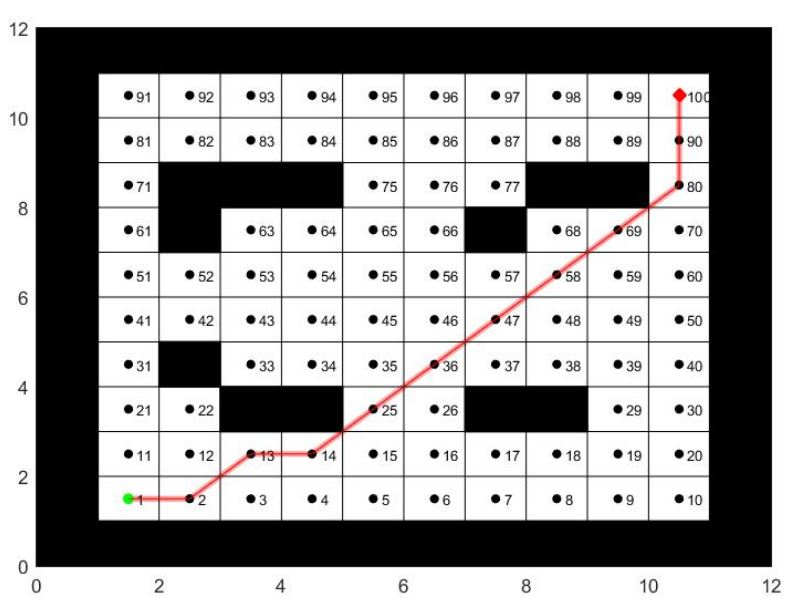
\includegraphics[width=0.5\textwidth]{mapa.jpg}
	\caption{Mapa y trayectoria generada para la validación en Webots \cite{baldizon_garcia_aplicaciones_2022}.}
	\label{fig2_5}
\end{figure}

\begin{figure}[H]
	\begin{subfigure}{0.5\textwidth}
		\centering
		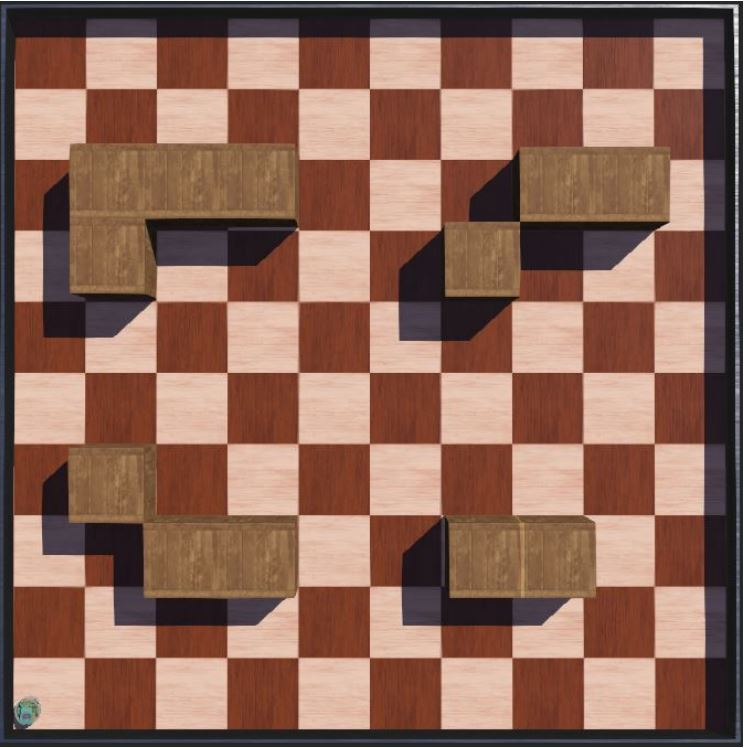
\includegraphics[width=0.9\linewidth]{pos_ini.jpg}
		\caption{Posición inicial.}
	\end{subfigure}
	\begin{subfigure}{0.5\textwidth}
		\centering
		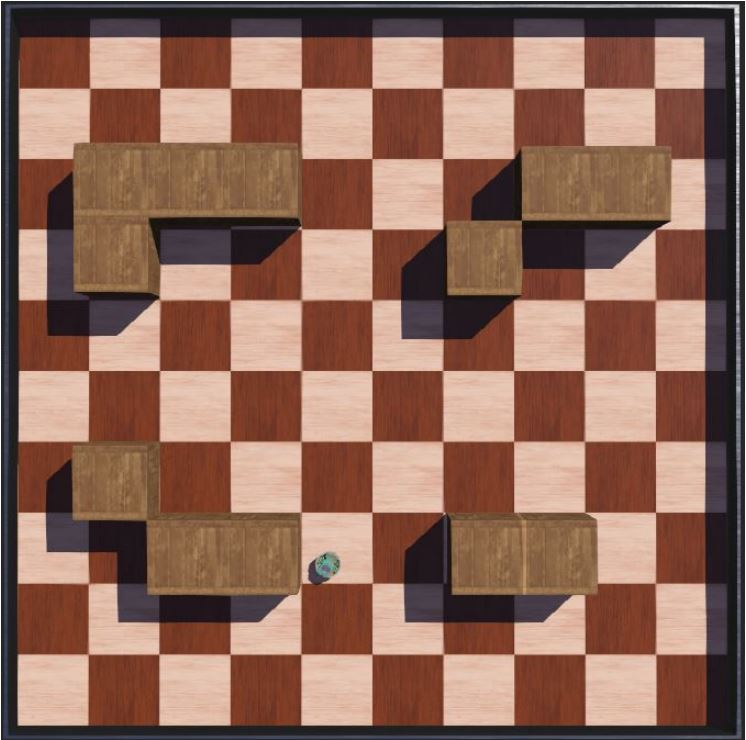
\includegraphics[width=0.9\linewidth]{pos_int1.jpg}
		\caption{Posición intermedia.}
	\end{subfigure}
	\begin{subfigure}{0.5\textwidth}
		\centering
		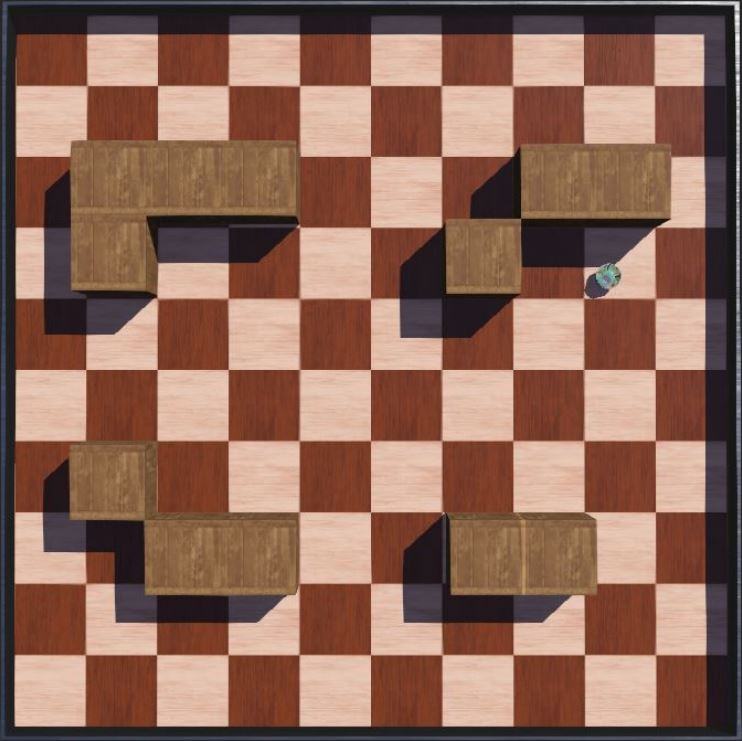
\includegraphics[width=0.9\linewidth]{pos_int2.jpg}
		\caption{Posición intermedia.}
	\end{subfigure}
	\begin{subfigure}{0.5\textwidth}
		\centering
		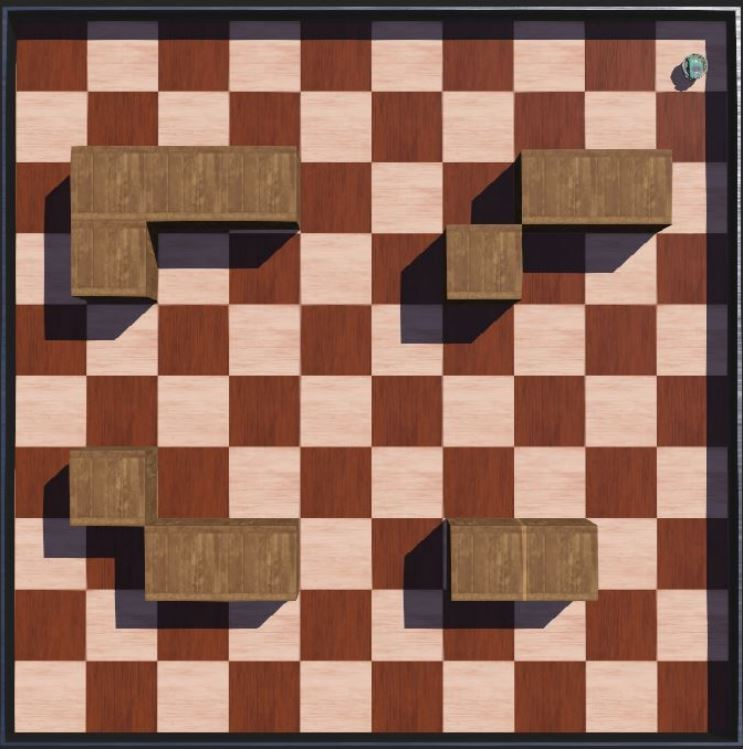
\includegraphics[width=0.9\linewidth]{pos_fin.jpg}
		\caption{Posición final.}
	\end{subfigure}
	\caption{Secuencia de movimientos del agente móvil para la evasión de obstáculos en Webots \cite{baldizon_garcia_aplicaciones_2022}.}
	\label{fig2_6}
\end{figure}


En \cite{godoy_lucero_desarrollo_2023} se desarrollaron y evaluaron algoritmos para el mapeo de entornos y generación de trayectorias utilizando sistemas robóticos multi-agente. Se enfocó en la implementación simulada de la combinación de tres algoritmos relacionados con la navegación autónoma en robots con tracción diferencial. Estos algoritmos abarcaron la exploración de entornos, el mapeo bidimensional de los mismos y la generación óptima de trayectorias. Para llevar a cabo la validación, se desarrollaron y simularon en Webots distintos escenarios de trabajo que incluían pasillos,  espacios abiertos y obstáculos tridimensionales. Estos entornos fueron reconstruidos,  de manera individual y colectiva, por agentes robóticos móviles con sensores de distancia integrados: cinco sensores frontales separados por un ángulo de 45 grados entre sí y un único sensor colocado en la parte trasera del vehículo.

\begin{figure}[H]
	\centering
	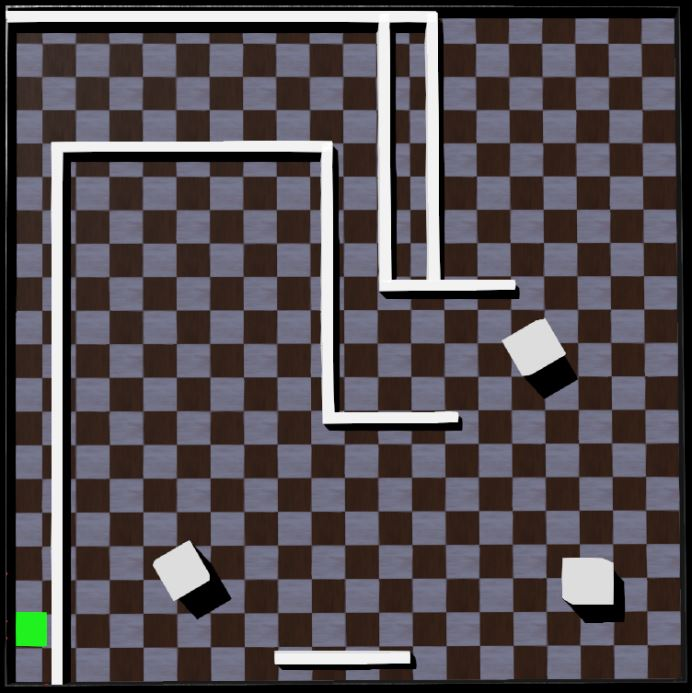
\includegraphics[width=0.6\textwidth]{escenario.jpg}
	\caption{Escenario simulado en Webots \cite{godoy_lucero_desarrollo_2023}.}
	\label{fig2_7}
\end{figure}

\begin{figure}[H]
	\centering
	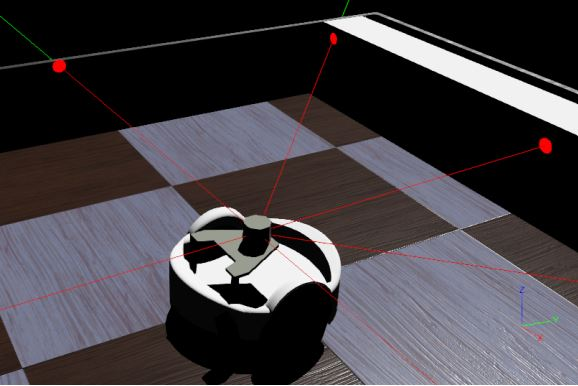
\includegraphics[width=0.5\textwidth]{exploracion.jpg}
	\caption{Puntos de visibilidad de los sensores integrados en el agente robótico móvil en Webots. \cite{godoy_lucero_desarrollo_2023}.}
	\label{fig2_8}
\end{figure}


En las simulaciones computarizadas, se observó que la integración de sensores a distancia tipo láser en lugar de los tipo sonar en los agentes resultaba más precisa y eficaz en la detección de obstáculos, asegurando trayectorias de exploración confiables y no redundantes. Además, se destacó que la disposición e interacción entre estos sensores influía en la capacidad del sistema para obtener una representación precisa del entorno. Se decidió combinar los datos provenientes de todos los sensores delanteros para compensar las limitaciones individuales de cada sensor, obteniendo una buena estimación y reconstrucción del entorno. La precisión en la distribución y disposición de los obstáculos en las estimaciones del espacio de trabajo permitieron el desarrollo y validación del algoritmo de planificación de trayectorias en mapas previamente explorados. Basándose en las validaciones simuladas de los algoritmos desarrollados, el autor recomienda dos sensores de distancia comerciales para la implementación física de estos algoritmos en futuros estudios. No obstante, se mencionaron ciertas limitaciones respecto a la representación exacta del entorno debido a la falta de información en ciertas áreas por el tiempo de simulación y colisiones recurrentes por obstáculos imprevistos, como la esquina de un obstáculo. 

\begin{figure}[H]
	\centering
	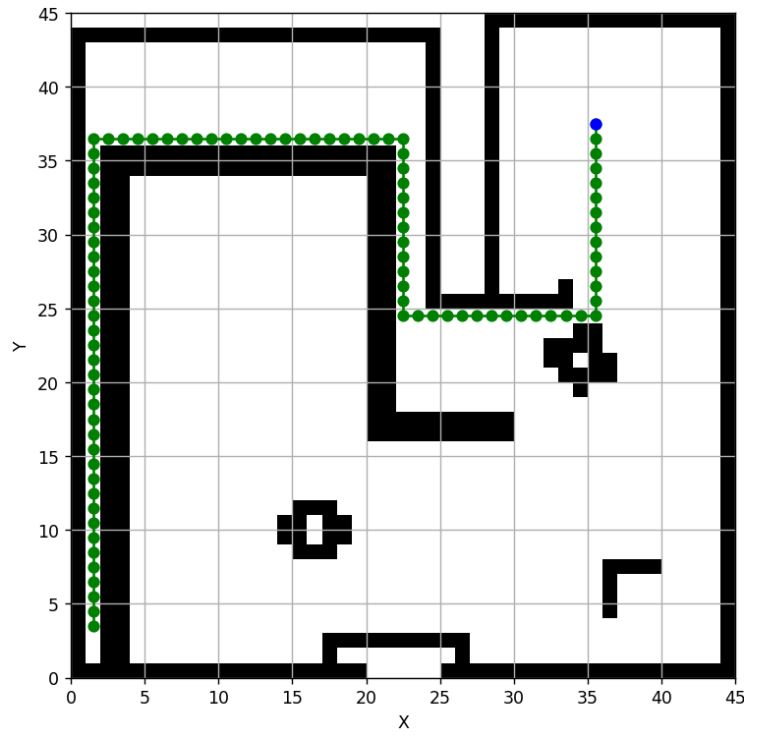
\includegraphics[width=0.6\textwidth]{mapeo.jpg}
	\caption{Espacio de trabajo estimado en exploración de 10 minutos, con planificación de trayectoria hacia su posición inicial de simulación  \cite{godoy_lucero_desarrollo_2023}.}
	\label{fig2_9}
\end{figure}

\section{Robotat}
En las instalaciones de la Universidad del Valle de Guatemala, se encuentra un laboratorio especializado en la experimentación robótica denominado Robotat. Inspirado en el Robotarium del Instituto de Tecnología de Georgia \cite{maderer_robotarium_nodate}, Estados Unidos, este espacio cuenta con una plataforma de acero blanca de 4.8 × 3.8 m, rodeada por el sistema de captura de movimiento OptiTrack. Dicho sistema está conformado por seis cámaras de alta precisión y baja latencia, diseñadas para capturar movimiento en tiempo real. Además, el laboratorio dispone de una red WiFi local que permite la comunicación entre los robots. Este entorno ha creado un ecosistema integral de aprendizaje, investigación y desarrollo práctico en el campo de la robótica \cite{barrera_robotat_nodate}.

En los sistemas de captura de movimiento, el uso eficiente de las cámaras es fundamental para procesar de manera óptima las imágenes obtenidas. En el caso del Robotat, el sistema OptiTrack utiliza marcadores reflectivos de plástico conocidos como marcadores pasivos para calcular con precisión la localización tridimensional de los objetos \cite{perafan_camilo_2022}. Estos marcadores reflejan la luz infrarroja emitida por las cámaras, lo que permite su detección dentro de la plataforma. Además, pueden adherirse a diversos objetos para rastrear su posición dentro del espacio 3D que abarca la plataforma, facilitando un seguimiento detallado y preciso de los movimientos.

\begin{figure}[H]
	\centering
	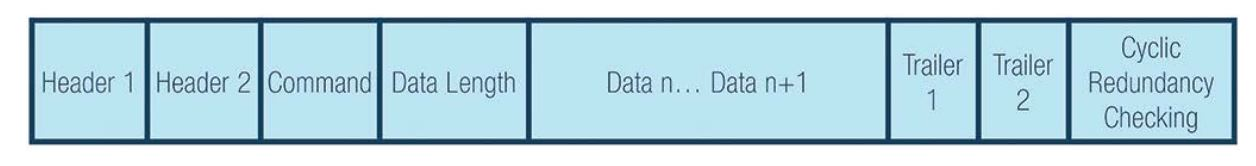
\includegraphics[width=0.6\textwidth]{uart_protocol.jpg}
	\caption{Robotat, laboratorio especializado en experimentación robótica.}
	\label{robotat}
\end{figure}